\section{Diseño de la arquitectura de la aplicación}
Antes de empezar con el desarrollo de la API y del sitio web se expondrá la arquitectura que se ha utilizado para el desarrollo de estos elementos.

\subsection{¿Qué es una arquitectura de software?}
Según el IEEE la arquitectura es la organización fundamental de un sistema compuesto por sus componentes, las relaciones que tienen unos con otros y con el entorno y los principios que guían su diseño y evolución.
\\Entendiendo sistema como un conjunto de componentes que se organizan para cumplir una determinada función o conjunto de funciones.
\\Un sistema existe para cumplir una o más misiones en su entorno.
\\El entorno o contexto determina la configuración y circunstancias en el desarrollo, las operaciones, la política y demás aspectos que puedan influenciar a un sistema.
\\La arquitectura de software es de vital importancia en el desarrollo de un sistema ya que determina su estructura conllevando un aspecto directo sobre la capacidad de este para satisfacer los requisitos y evolución de un proyecto.

\subsubsection{¿Por qué es importante definir una arquitectura software?}
Definir una arquitectura de software presenta varias ventajas. Entre ellas se encuentran las siguientes:
\begin{itemize}
    \item \textbf{Independencia de los frameworks}: Una arquitectura puede ser definida en múltiples frameworks y lenguajes pues no depende de ellos.
    \item \textbf{Independencia de las reglas de negocio}: Las reglas de negocio no se verán alteradas por el cambio de arquitectura software.
\end{itemize}


\subsection{Clean Architecture o Arquitectura Limpia}
Es un conjunto de principios cuya finalidad principal es ocultar los detalles de implementación a la lógica de dominio de la aplicación.
\\Gracias a esto puede mantenerse la lógica de la aplicación aislada de forma que sea más mantenible a lo largo del tiempo.
\\Para explicar qué es la arquitectura limpia se dispone del gráfico \ref{clean_architecture_diagram}.

\begin{figure}[h]
    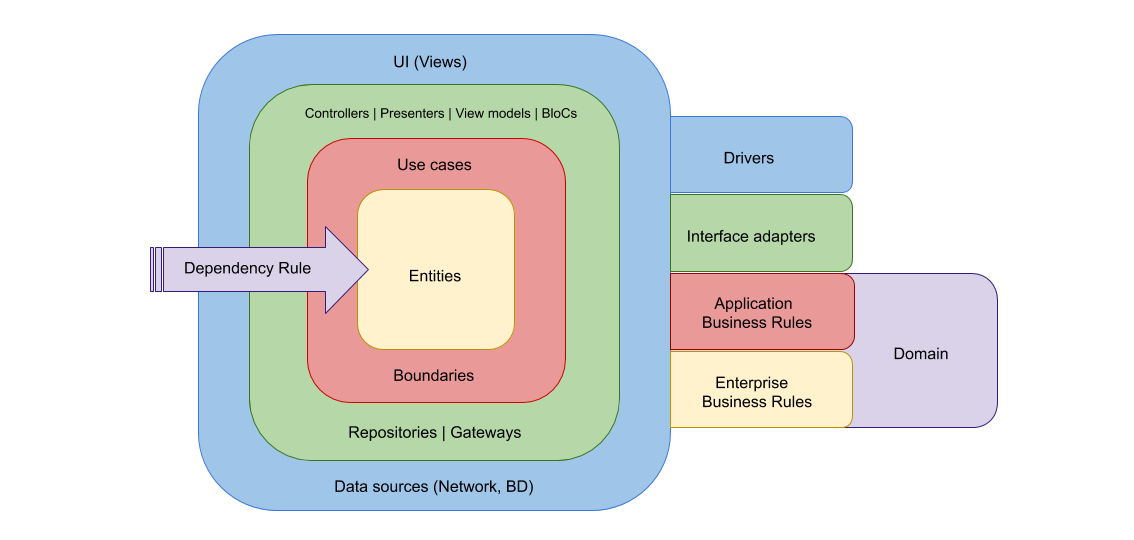
\includegraphics[width=\textwidth,height=\textheight,keepaspectratio]{../complemento/clean_architecture.png}
    \caption{Clean Architecture}\label{clean_architecture_diagram}
\end{figure}

Puede observarse que la estructura del diagrama está formada por capas. Las capas representan distintos conjuntos que componen el sistema.
\\Dentro de la figura puede verse una flecha en la que aparece escrito ``Dependency Rule'', en español, regla de dependencia. Significa el sentido que tomarán los distintos componentes de la aplicación. En este caso de afuera hacia dentro. Los componentes más externos dependen de los más internos y las entidades o el dominio de la aplicación depende de ella misma.
\\En el momento de la separación de funcionalidades hay que tener en cuenta que el sistema se divide en tres partes. La web, la API y la base de datos.

\subsubsection{Entidades}
Las entidades representan las piezas básicas de la aplicación. Estas serían las tablas del diagrama de la base de datos. Cada una de las tablas conforma un tipo de datos. Pueden tener dependencias entre ellos pero nunca van a tener dependencias externas.
\\Por eso es lo primero que se define ya que si hay que cambiarla habría que cambiar los elementos que dependieran de ella.

\subsubsection{Casos de uso}
Los casos de uso están definidos en la API, que es la que gestiona todos los procesos internos que pueden realizarse con los datos, desde la solicitud de préstamos hasta dar de alta a un usuario.

\subsubsection{Controladores, presentadores y vistas de los modelos}
Este conjunto está definido por las herramientas que ayudan a solicitar y adaptar la información más interna de la aplicación. También en esta parte tenemos las interfaces las cuales ayudan a adaptar los datos que llegan de los casos de usos para poder interpretarlos.

\subsubsection{Vistas y fuentes externas}
Aquí están los frameworks, los adaptadores de red, el servidor de la base de datos y las vistas que es la forma en que se estructura y diseña la información para que se muestre al usuario.